\chapter{Introduction}\label{chap:introduction}
\par Ever since I was a child, I liked playing with Rubik's Cubes. I was told by my uncle that there is a lot of mathematics behind this fascinating toy, such as the Rubik's Cube can be viewed as a group. Now, I am at the age where I gathered enough skills to understand the complexities of the Rubik's Cube. In this thesis, I investigate how to link Rubik's Cube with cryptography, a subject I obsessed with since sophomore year of college.
\par We start with discussing what cryptography is and listing motivations for us to integrate Rubik's Cubes with encryption protocols. While presenting design ideas of the Rubik's Cube encryption, we consider limitations and make corresponding improvements. Then, under the formal definition of security, we test if our Rubik's Cube encryption is well designed, and tweak it to make the encryption protocol better under the definition of security. Finally, we illustrate some known structures of the Rubik's Cube groups and introduce a Rubik's Cube key exchange protocol which has a similar structure that the Diffie-Hellman key exchange protocol uses.

\section{What is cryptography}
\par The definition of cryptography\cite{cryptography} given in the Merriam-Webster dictionary is ``\textit{secret writing}''. This is historically precise, since in ancient times, people applied the idea of cryptography solely to enable secret communication. Most ancient cryptography schemes, as well as some modern ones look like some kind of puzzle. Yet creating and breaking the scheme would rely on how well you can manipulate the puzzle.
\par One basic scheme is the Substitution cipher, which replaces each unit of the plaintext to form the ciphertext. If we are working with English, then each unit of plaintext will be a letter.
\begin{figure}[ht]
    \centering
    \setlength\tabcolsep{3pt}
        \begin{tabular}{cccccccccccccccccccccccccc}
        A & B & C & D & E & F & G & H & I & J & K & L & M & N & O & P & Q & R & S & T & U & V & W & X & Y & Z \\
        $\downarrow$ & $\downarrow$ & $\downarrow$ & $\downarrow$ & $\downarrow$ & $\downarrow$ & $\downarrow$ & $\downarrow$ & $\downarrow$ & $\downarrow$ & $\downarrow$ & $\downarrow$ & $\downarrow$ & $\downarrow$ & $\downarrow$ & $\downarrow$ & $\downarrow$ & $\downarrow$ & $\downarrow$ & $\downarrow$ & $\downarrow$ & $\downarrow$ & $\downarrow$ & $\downarrow$ & $\downarrow$ & $\downarrow$ \\
        Z & E & B & R & A & S & C & D & F & G & H & I & J & K & L & M & N & O & P & Q & T & U & V & W & X & Y \\
    \end{tabular}
    \caption{Map letter to letter}\label{fig:replace-letter-by-letter}
\end{figure}
One trivial example could be substituting each letter to another unique letter as displayed in Figure~\ref{fig:replace-letter-by-letter}. If we encrypt the sentence \textit{``life is like a box of chocolates''} with the relations specified in Figure~\ref{fig:replace-letter-by-letter}, we get \textit{``ifsafpifhazelwlsbdlblizqap''} back as the ciphertext. Correspondences between plaintext and ciphertext can be very creative as long as the communicating parties hold the same information. 
\begin{figure}[ht]
    \centering
    \setlength\tabcolsep{3pt}
    \resizebox{\linewidth}{!}{
        \begin{tabular}{cccccccccccccccccccccccccc}
            A & B & C & D & E & F & G & H & I & J & K & L & M & N & O & P & Q & R & S & T & U & V & W & X & Y & Z \\
            $\downarrow$ & $\downarrow$ & $\downarrow$ & $\downarrow$ & $\downarrow$ & $\downarrow$ & $\downarrow$ & $\downarrow$ & $\downarrow$ & $\downarrow$ & $\downarrow$ & $\downarrow$ & $\downarrow$ & $\downarrow$ & $\downarrow$ & $\downarrow$ & $\downarrow$ & $\downarrow$ & $\downarrow$ & $\downarrow$ & $\downarrow$ & $\downarrow$ & $\downarrow$ & $\downarrow$ & $\downarrow$ & $\downarrow$ \\
            \faAsterisk{} & \faBank{} & \faCube{} & \faDiamond{} & \faEnvelope{} & \faFilm{} & \faGear{} & \faHashtag{} & \faImage{} & \faJoomla{} &\faKey{} & \faLeaf{} & \faMagnet{} & \faNavicon{} & \faOpenid{} & \faPaperPlane{} & \faQrcode{} & \faRandom{} & \faSave{} & \faTag{} &\faUser{} & \faVideoCamera{} & \faWifi{} & \faXing{} & \faYoutubePlay{} & \faTv{}
        \end{tabular}
    }
    \caption{Map letter to icon}\label{fig:replace-letter-by-icon}
\end{figure}
The ``creative'' example is shown in Figure~\ref{fig:replace-letter-by-icon}, where we are replacing letters by icons which are completely irrelevant. We can encrypt the same sentence \textit{``\;life is like a box of chocolates''} again and this time we get ``\faImage{} \faFilm{} \faSave{} \faAsterisk{} \faFilm{} \faPaperPlane{} \faImage{} \faFilm{} \faHashtag{} \faAsterisk{} \faTv{} \faEnvelope{} \faLeaf{} \faWifi{} \faLeaf{} \faSave{} \faBank{} \faDiamond{} \faLeaf{} \faBank{} \faLeaf{} \faImage{} \faTv{} \faQrcode{} \faAsterisk{} \faPaperPlane{}\;'' back.
\par Intuitively, we know the security of substitution cipher is based on the fact that the correspondence between plaintext and ciphertext is unknown to the attacker. Although we may find the second substitution to be more abstract, the brute force attack or frequency analysis will be equally effective on both.
\par Historically, the biggest motivation for people to research in this field, and most applications, were military related. Thus cryptography seemed far away from most people's daily life. However, cryptography has primarily changed since the invention of computers and the internet. It has merged deeply into our everyday life though you may not have noticed. Whenever you log in your email account or when you purchase an item from an online shop, you have undoubtedly used cryptography. While you are communicating with the web servers, your email account password or credit card number will first be encrypted and then sent through the networks. If that critical information were never encrypted, anyone who can monitor your network would be able to retrieve your private information.
\par While secure communication is still the major motivation of cryptography, the study of cryptography has developed other related branches that are equally important. Some of the noticeable branches are key exchanging protocols, message authentication code, hash functions and more. Later in this writing, we will discover more about key exchanging protocols as they are crucial components of symmetric encryptions. Message authentication code, usually shorten as MAC, is used to confirm that the message came from the stated sender and has not been modified. Hash function is one commonly used tool to build valid MACs.
\par Computers have also brought us ample computational powers. In modern times, a 30 dollars Raspberry Pi can perform an exhaustive attack on the substitution cipher on 26 English letters showed in our first example in the time it takes to make a cup of coffee. Thus, deviating from studying the art of clever puzzles, modern cryptography makes extensive use of mathematics, including fields such as abstract algebra, number theory, statistics, combinatorics, and computational complexities.
\par In a nutshell, cryptography has gone from the set of clever puzzles concerned with ensuring secret communication for the military to science that provides security for ordinary people across the globe. Modern cryptography heavily relies on mathematical theory and computer science practice. Cryptographic protocols are designed around some computational hardness assumptions, meaning that theoretically, it is possible for one to break such protocol, but it is infeasible to do so by any practical means.

\section{Rubik's Cube and cryptography}
% ---------------------- Figure for a solved Rubik's Cube ----------------------
\begin{wrapfigure}{r}{6cm}
    \centering
    \RubikFaceUpAll{Y}
    \RubikFaceFrontAll{G}
    \RubikFaceRightAll{O}
    \ShowCube{5cm}{0.9}{\DrawRubikCubeRU}
    \caption{Rubik's Cube}\label{fig:solved-cube}
\end{wrapfigure}
% ------------------------------------------------------------------------------
\par Rubik's Cube, as shown in Figure~\ref{fig:solved-cube}, is a three dimensional puzzle invented in 1974 by Hungarian professor Erno Rubik. The most common Rubik's Cube has six faces. The faces of the cube are covered by the following solid colors: white, red, blue, yellow, orange and green. For a solved cube, the white face is always opposite to the yellow face, red is opposite to orange and blue is opposite to green. As shown in Figure~\ref{fig:solved-cube}, the Rubik's Cube has three small cubes on each side. We say that this is a 3 by 3 by 3 cube, or that it is a cube with side length of 3. Clearly each face of the cube includes nine squares. In future discussions, we will call those squares \textit{cubies}.
\par After years of developing, Rubik's Cubes now exist in many forms. For the six faced cubes, their side lengths may vary from 2 to 13 or even larger number. However, since their structures are similar, they share a lot of properties in common. For example, regardless of the side length, all six faced cubes can be solved in an almost identical fashion. 
\begin{figure}[ht]
    \centering
    \begin{minipage}{0.45\textwidth}
        \centering
        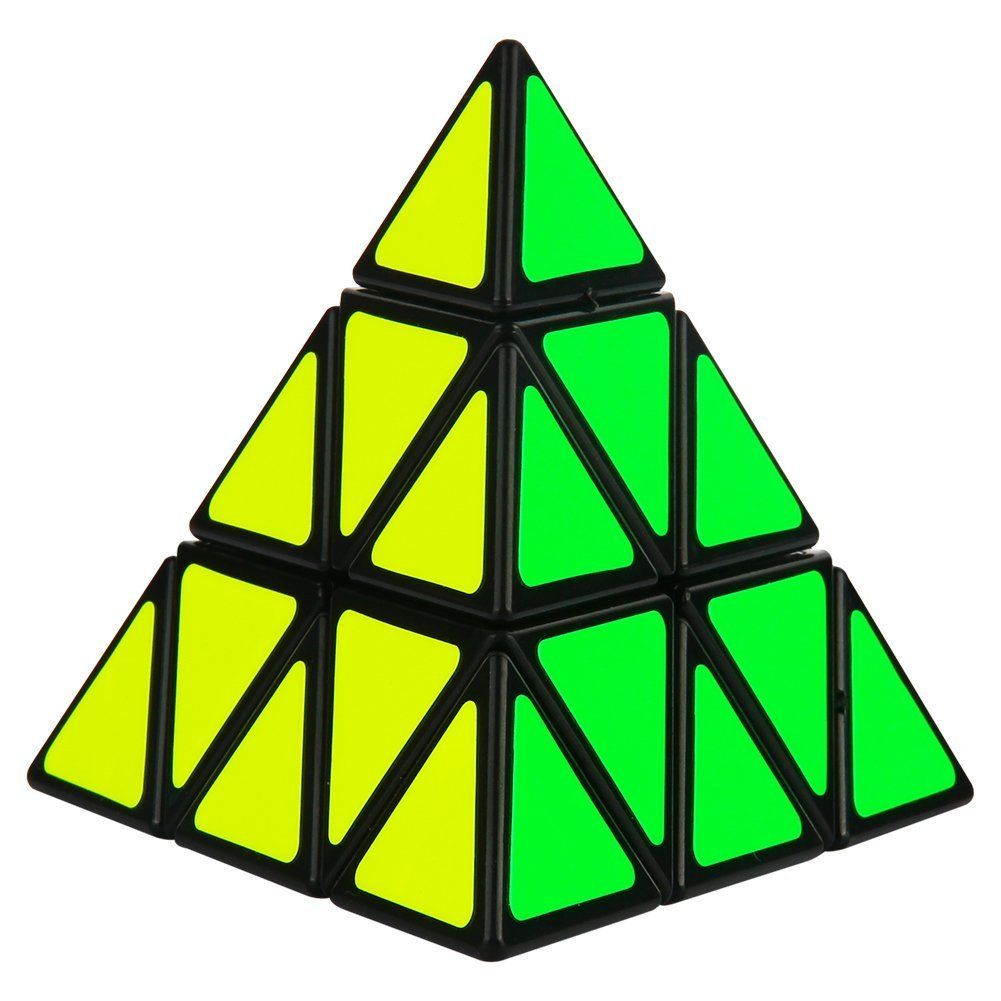
\includegraphics[width=.6\linewidth]{figures/introduction/pyraminx_cube.jpg}
        \caption{A solved pyraminx cube}\label{fig:pyraminx-cube}
    \end{minipage}
    \begin{minipage}{0.45\textwidth}
        \centering
        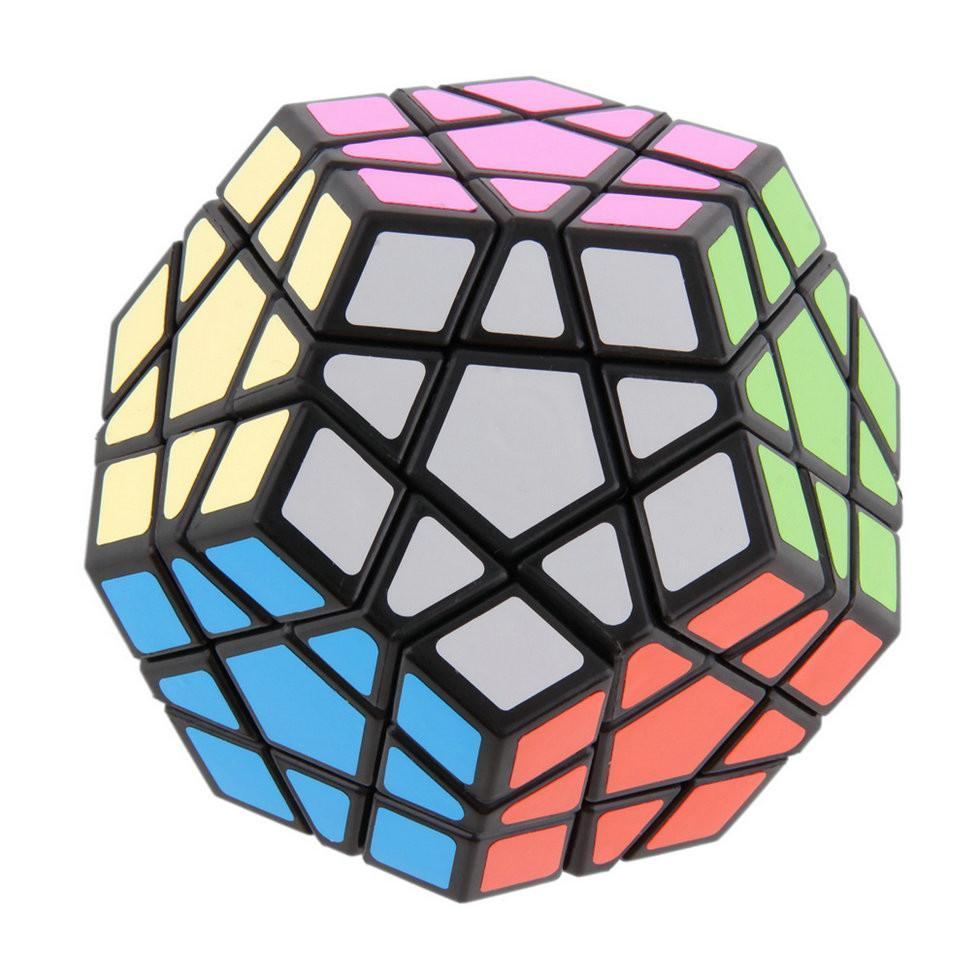
\includegraphics[width=.6\linewidth]{figures/introduction/pentagon_cube.jpg}
        \caption{A solved pentagon cube}\label{fig:pentagon-cube}
    \end{minipage}
\end{figure}
We will refer Rubik's Cube with side length $n$ as $C_n$. For instance, the normal 3 by 3 by 3 Rubik's Cube will be denoted as $C_3$. Also when $n$ is an odd number we will call $C_n$ an odd cube and when $n$ is an even number we will call $C_n$ an even cube. Further more, Rubik's Cubes also have other structures; ``cubes'' with four or twelve faces as listed in Figure~\ref{fig:pyraminx-cube} and Figure~\ref{fig:pentagon-cube} have also been made in production.
\par Why would we relate Rubik's Cubes and cryptography? As we mentioned in the last section, cryptographic protocols are designed around some hard problems, and Rubik's Cubes are known to be hard to solve. One may argue that this is not true since the best human players can solve a 3 by 3 by 3 cube in about 6 seconds. By carefully following the developed algorithms, anyone can solve a well shuffled Rubik's Cube within a couple of minutes. \par Suppose we play the Rubik's Cube differently; after shuffling the cube, we give it to a player without letting him/her observe it. Therefore, to solve the puzzle, the player has to guess and shuffle it randomly. Then, the player needs to confirm with a judge to see if the cube is solved. The player wins if the cube is solved, but if the cube is not solved, it will be reversed back to its beginning state and the player has to guess again. Under this setting, the Rubik's Cube will become much harder to solve because the player has to go through an enormous amount of possible cases. 
\par This is essentially what we will do in Chapter~\ref{chap:encryption}. We place our plaintext on the cube and remove the colors from the faces and then shuffle the cube. Let us consider each different shuffling result of the Rubik's Cube as a state. The most common cube $C_3$ has over 43 quintillion different states. It will take decades for a powerful desktop to run through all of them. Hence it will almost be impossible for a human player to run through all possibilities and guess if the cube is correctly solved. Also, when the side length of a Rubik's Cube grows, the number of states the cube produces will grow significantly fast. Being such a powerful device, Rubik's Cubes can be used to design schemes that are safe against exhaustive search attacks. In addition, we can algebraically view Rubik's Cubes as groups. The nice properties of groups are widely used in cryptography, and we will see how to use the group structure of Rubik's Cube to define a key exchange protocol.

\section{Preliminaries}
\par First let's take a look at \textbf{\textit{Kerckhoffs's principle}}:
\begin{quote}
    \textit{The cipher method must not be required to be secret, and it must be able to fall into the hands of the enemy without affecting the security of the cipher method.}
\end{quote}
This principle tells us that the security of an encryption protocol does not rely on the encryption protocol procedures being unknown. One may wonder how do we obtain the security while the eavesdropper knows all the details. But there is one thing the eavesdropper does not know, which is the \textbf{\textit{key}}. In fact, the security of all classical encryption schemes depends on the key shared by the communicating parties being unknown by the eavesdropper. For our substitution cipher example, we consider the correspondence between plaintext and ciphertext as the key. Like we said, the security of substitution cipher depends on the key being secret. This scenario is known as the \textit{private-key} setting.
\par Formally, to create a private-key encryption scheme, we need to specify a message space $\mathcal{M}$. This message space $\mathcal{M}$ defines the set of ``legal'' messages. Taking the substitution cipher described in Figure~\ref{fig:replace-letter-by-letter} as an example, a ``legal'' message could be any combination of English letters without spaces or punctuations, regardless of if it has any actual meaning. In contrast, any message containing a Greek letter will make the message  ``illegal''. Along with defining the message space, we need three algorithms for a private-key encryption scheme, which are \textbf{Gen}, \textbf{Enc} and \textbf{Dec}:
\begin{itemize}
    \item \textbf{Gen} is the procedure for generating keys. It is a probabilistic algorithm that outputs a key $k$ with desired length according to some distribution.
    \item \textbf{Enc} is the procedure for encrypting the message. It takes a key $k$ and a message $m \in \mathcal{M}$ as inputs. Then it uses $k$ to encrypt $m$ and outputs ciphertext $c$. We denote this process by \textbf{Enc}$_k(m)$.
    \item \textbf{Dec} is the procedure for decrypting the message. It takes a key $k$ and a ciphertext $c$ as inputs. Then it uses $k$ to decrypt $c$ and outputs plaintext $m$. We denote this process by \textbf{Dec}$_k(c)$.
\end{itemize}
\par It is worth noting that the set of all possible keys output by the key-generation algorithm is called the key space and is denoted by $\mathcal{K}$. In most cases, \textbf{Gen} randomly picks one key from the key space uniformly.
\par With these algorithms, we can move on to construct the set of legal encryption schemes. One requirement an encryption scheme must satisfy is defined as the following.
\begin{definition} \textbf{The correctness of an encryption scheme} \\
    For any encryption scheme $\Pi = (\textbf{Enc}, \textbf{Gen}, \textbf{Dec})$ and for every $k$ generated by \textbf{Gen} and every message $m \in \mathcal{M}$, it must hold that \[\textbf{Dec}_k(\textbf{Enc}_k(m)) = m\]
\end{definition}
\par This simply means that we accurately decrypt any encrypted message when we hold the correct key. To provide an example of a valid encryption scheme, we simply define $\Pi = (\textbf{Enc}, \textbf{Gen}, \textbf{Dec})$, where \textbf{Enc}$_k(m) = m$ and \textbf{Dec}$_k(c) = c$. In words, both \textbf{Enc} and \textbf{Dec} do not modify the input string regardless of what the key $k$ is. So $\Pi$ is a valid encryption scheme as it satisfies the correctness of an encryption scheme. But obviously, $\Pi$ is not a secure scheme. As we explore more about using Rubik's Cube to perform encryption, we will also explore what it means for an encryption scheme to be secure.